% Provenance (never printed): see sources/outline_sources.md (Year 1:
% the Solar System, planetology). Kepler's laws, the moment of inertia and
% the Stefan--Boltzmann law are owned by the physics series and recalled
% here; the equilibrium temperature and the Bond albedo are re-founded from
% Book 2 grade 10. Curves computed in figdata/bachelor-1/planet_table.py;
% numbers of the exercises and problem in the Book 3 scratch calculator
% ch03.py.
\chapter{比较行星学}\label{ch:b1:comparative-planetology}

金星与地球几乎是一对孪生星：金星的半径为地球的 \qty{95}{\percent}，
质量为地球的 \qty{81}{\percent}。然而地球有海洋、
氮氧大气与运动的板块，而金星的表面藏在云层之下，
表面温度达 \qty{737}{K}，比任何厨房烤箱都热，并受
压力达 \qty{92}{bar} 的二氧化碳大气挤压。火星大小约为地球的一半，
大气稀薄而寒冷，有巨型火山和峡谷，却没有运动的
板块。更远处的木星和土星
主要由氢和氦组成；天王星和海王星则主要是水、
甲烷和氨的冰。比较各行星，是检验我们对地球的
认识是否可靠的唯一途径：地球内部为何分层，气候
为何温和，为何唯独它有板块构造。本章称量并测量
各行星，依据其密度及质量分布推断内部结构，
比较其温度与大气，最后以卫星和小天体收尾，
这些天体保存着太阳系
早期的记录。
% ledger: nasa:venus, earth:Rmean, earth:mass, nasa:uranus-structure

\begin{recall}
行星沿椭圆绕太阳运行，卫星的周期平方
与其半长轴的立方成正比（开普勒第三定律，
见物理系列本科一年级分册，其中定义了固体的
转动惯量；均匀球体有 $I = \tfrac25MR^2$），黑体
每单位面积辐射 $\sigma T^4$（本科二年级）。太阳系及其
\omterm{def:b1:comparative-planetology:planet-types}{类地行星}与\omterm{def:b1:comparative-planetology:planet-types}{巨行星}已在第 1 册（六年级）中介绍，
行星的反照率与\omterm{def:b1:comparative-planetology:equilibrium-temperature}{平衡温度}已在第 2 册（十年级）中学过，
温室效应则在第 1 册（九年级）中学过。
\end{recall}

\begin{omfigure}
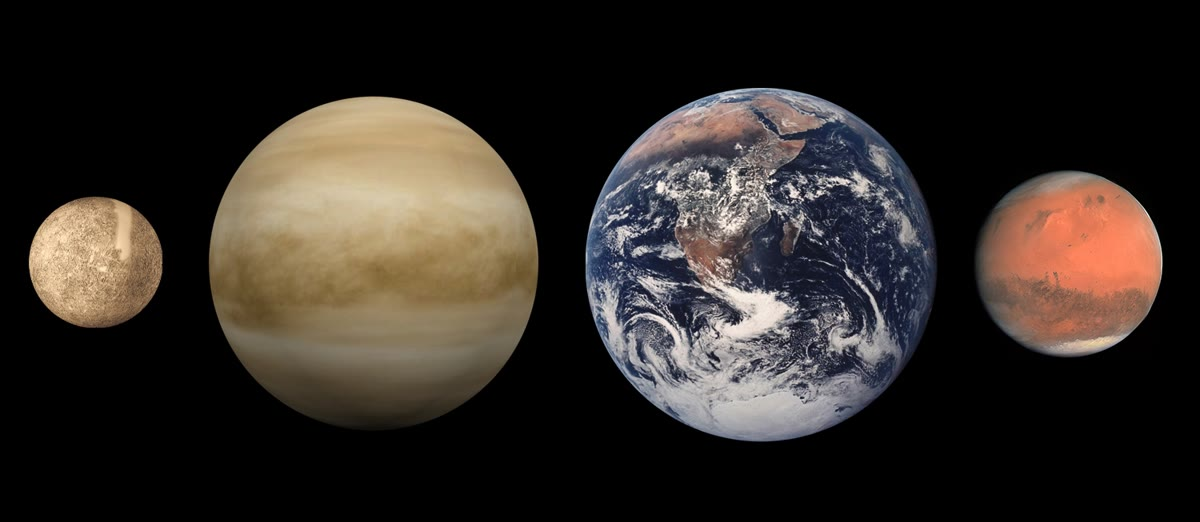
\includegraphics[width=0.85\linewidth]{images/book3/b1-terrestrial-planet-sizes.jpg}

{\small 四颗\omterm{def:b1:comparative-planetology:planet-types}{类地行星}按比例绘制，自左至右依次为水星、
金星、地球和火星（距离不按比例；金星为可见光下所见，
其表面被云层遮盖）。NASA，公有领域。}
% ledger: commons:terrestrial-sizes
\end{omfigure}

\section{称量与测量行星}

行星的半径可由其视直径和距离测得，
对于被探测器造访的行星，也可由雷达和激光测高获得。
其质量则较难测定：只能通过行星对
其他物体施加的引力来感知。

\begin{method}[由卫星轨道求行星的质量]\label{met:b1:comparative-planetology:mass}
设一颗质量可忽略的卫星在近似圆形的轨道上运行，
轨道半径（半长轴）为 $a$，恒星周期为 $T$，绕质量为 $M$ 的行星运动：
\begin{enumerate}
  \item 将 $a$ 化为米，$T$ 化为秒；
  \item 由开普勒第三定律得 $GM = 4\pi^2a^3/T^2$：此乘积是
        轨道所测得的量，且其精度远高于 $G$ 本身；
  \item 除以 $G = \qty{6.6743e-11}{m^3.kg^{-1}.s^{-2}}$，即得 $M$。
\end{enumerate}
没有卫星的行星（水星、金星）同样可以
根据经过它的探测器的轨道或偏折来称量。
\end{method}

\begin{example}
木卫一是木星最内侧的大型卫星，其轨道半长轴为 $a = \qty{421.8e3}{km}$，
运行周期为 \num{1.769138} 天，即 $T = \qty{152854}{s}$。于是
\[
  GM = \frac{4\pi^2\times(\qty{4.218e8}{m})^3}{(\qty{152854}{s})^2}
  = \qty{1.268e17}{m^3.s^{-2}}, \qquad
  M = \frac{\num{1.268e17}}{\num{6.6743e-11}} = \qty{1.900e27}{kg},
\]
计算结果与木星的表列质量 \qty{1.898e27}{kg} 相符，
相差不超过 \qty{0.1}{\percent}。木卫一自身的质量仅为木星的 \num{4.7e-5}，可忽略不计；
略偏大的部分来自木星的赤道隆起，它对近距卫星的
吸引力比同质量的球体略强。
% ledger: nasa:io, nasa:jupiter, const:G
\end{example}

由质量和半径可求得平均密度 $\bar\rho =
3M/(4\pi R^3)$，它是了解行星由何构成的第一条线索。行星的密度
分为两组（见下图）：水星、金星、地球和
火星的密度约在 \num{3900} 与 \qty{5500}{kg.m^{-3}} 之间，
比任何常见岩石都致密；四颗外侧的\omterm{def:b1:comparative-planetology:planet-types}{巨行星}则
介于 \num{690} 与 \qty{1640}{kg.m^{-3}} 之间，接近水的密度，土星
甚至低于水的密度。
% ledger: planet:Mercury.density, planet:Mars.density, planet:Earth.density, planet:Saturn.density, planet:Neptune.density

\begin{omfigure}
\begin{tikzpicture}
\begin{axis}[omrecord, width=0.86\linewidth, height=6.2cm, xmode=log,
  xmin=800, xmax=150000, ymin=0, ymax=6300, xlabel={赤道半径（km）},
  ylabel={平均密度（\unit{kg.m^{-3}}）}, tick label style={font=\scriptsize},
  label style={font=\small}]
\addplot[only marks, mark=*, mark size=2.4pt, brown!70!black] table[x=R_km, y=density,
  restrict expr to domain={\thisrow{idx}}{0:2}] {figdata/out/bachelor-1-planet_table-bodies.dat};
\addplot[only marks, mark=*, mark size=2.4pt, brown!70!black] table[x=R_km, y=density,
  restrict expr to domain={\thisrow{idx}}{4:4}] {figdata/out/bachelor-1-planet_table-bodies.dat};
\addplot[only marks, mark=*, mark size=2.4pt, orange!85!black] table[x=R_km, y=density,
  restrict expr to domain={\thisrow{idx}}{5:6}] {figdata/out/bachelor-1-planet_table-bodies.dat};
\addplot[only marks, mark=*, mark size=2.4pt, omDef] table[x=R_km, y=density,
  restrict expr to domain={\thisrow{idx}}{7:8}] {figdata/out/bachelor-1-planet_table-bodies.dat};
\addplot[only marks, mark=o, mark size=2.4pt, black!60] table[x=R_km, y=density,
  restrict expr to domain={\thisrow{idx}}{3:3}] {figdata/out/bachelor-1-planet_table-bodies.dat};
\addplot[only marks, mark=o, mark size=2.4pt, black!60] table[x=R_km, y=density,
  restrict expr to domain={\thisrow{idx}}{9:9}] {figdata/out/bachelor-1-planet_table-bodies.dat};
\addplot[black!40, densely dashed] coordinates {(800,1000) (150000,1000)};
\begin{scope}[font=\scriptsize]
\node[left] at (axis cs:2439.5,5429) {水星};
\node[below left] at (axis cs:6052,5243) {金星};
\node[above] at (axis cs:6378,5514) {地球};
\node[left] at (axis cs:3396,3934) {火星};
\node[left] at (axis cs:1737.5,3340) {月球};
\node[right] at (axis cs:1188,1850) {冥王星};
\node[above] at (axis cs:71492,1326) {木星};
\node[left] at (axis cs:60268,687) {土星};
\node[right] at (axis cs:25559,1270) {天王星};
\node[above] at (axis cs:24764,1638) {海王星};
\node[above left, black!60] at (axis cs:150000,1000) {水};
\end{scope}
\end{axis}
\end{tikzpicture}

{\small 八颗行星的平均密度随半径的变化（对数坐标）
（实心：\omterm{def:b1:comparative-planetology:planet-types}{类地行星}、\omterm{def:b1:comparative-planetology:planet-types}{气态巨行星}、\omterm{def:b1:comparative-planetology:planet-types}{冰巨星}），月球与冥王星（空心
圆）。数据来自 NASA 行星概况表。}
% ledger: planet:Mercury.diameter, planet:Venus.diameter, planet:Earth.diameter, planet:Moon.diameter, planet:Mars.diameter, planet:Jupiter.diameter, planet:Saturn.diameter, planet:Uranus.diameter, planet:Neptune.diameter, planet:Pluto.diameter, planet:Mercury.density, planet:Venus.density, planet:Earth.density, planet:Moon.density, planet:Mars.density, planet:Jupiter.density, planet:Saturn.density, planet:Uranus.density, planet:Neptune.density, planet:Pluto.density
\end{omfigure}

仅凭平均密度无法区分一颗由单一致密物质构成的行星与
一颗中心极为致密、外层较轻的行星。还需第二个量，
即质量在中心与表层之间如何分布。

\begin{definition}[转动惯量因子]\label{def:b1:comparative-planetology:moi}
称行星的\emph{转动惯量因子}\index{转动惯量因子}为
一个数：
\[
  C = \frac{I}{MR^2} ,
\]
式中 $I$ 为行星绕自转轴的转动惯量，$M$ 为质量，
$R$ 为平均半径。均匀球体有 $C = \tfrac25 = 0.4$；
密度向中心增大的行星有 $C < 0.4$，
且质量越集中于中心，此值越小。
\end{definition}

转动惯量由自转轴在太阳引力作用下的缓慢进动测得，
并结合行星引力场的扁率。
数值很能说明问题：月球 $C = 0.394$，
近乎均匀；火星 $0.366$ 与地球 $0.3308$ 明显
分层；木星 $0.254$ 与土星 $0.210$ 的大部分质量
都集中在其中心附近。
% ledger: nasa:moon, nasa:mars, earth:MoI, nasa:jupiter, nasa:saturn

\section{行星由什么构成}

\begin{definition}[类地行星与巨行星]\label{def:b1:comparative-planetology:planet-types}
称\emph{类地行星}\index{类地行星}为主要由硅酸盐岩石和铁构成、
具有固体表面的行星，包括水星、金星、
地球和火星。称\emph{巨行星}\index{巨行星}为质量远大于地球的行星，
主要由轻元素及其
化合物构成，且没有固体表面。称\emph{气态巨行星}\index{气态巨行星}为
主要由氢和氦构成的巨行星：木星和土星。
称\emph{冰巨星}\index{冰巨星}为主要由
天文学家所称“冰”的化合物——水、甲烷和氨——构成、外层包有氢和氦的巨行星：
天王星和海王星。
\end{definition}

探测器与望远镜所测得的大气证实了这一划分。
木星大气中氢占 \qty{89.8}{\percent}，氦占 \qty{10.2}{\percent}，
按体积计；土星则为 \qty{96.3}{\percent} 与 \qty{3.25}{\percent}；
对天王星，至少 \qty{80}{\percent} 的质量为高温致密的流体，
由水、甲烷和氨组成，位于一个小的岩质核心之上。\omterm{def:b1:comparative-planetology:planet-types}{气态巨行星}的平均
密度仍然很低，尽管其中心受到强烈压缩，原因是氢是最轻的元素；\omterm{def:b1:comparative-planetology:planet-types}{冰巨星}
比土星更致密，因为其中的冰比氢重。
% ledger: nasa:jupiter, nasa:saturn, nasa:uranus-structure

\omterm{def:b1:comparative-planetology:planet-types}{类地行星}与地球一样分层：富铁地核，
其上为硅酸盐地幔和薄地壳。能同时利用
两个实测数值（平均密度与\omterm{def:b1:comparative-planetology:moi}{转动惯量因子}）的最简单模型，
具有两层结构。

\begin{proposition}[两层结构的行星]\label{prop:b1:comparative-planetology:two-layer}
将半径为 $R$ 的行星看作半径为 $xR$ 的地核，密度均匀
为 $\rho_c$，置于密度均匀为 $\rho_m$ 的地幔之中。其平均密度与
\omterm{def:b1:comparative-planetology:moi}{转动惯量因子}分别为
\[
  \bar\rho = \rho_m + (\rho_c - \rho_m)\,x^3 , \qquad
  C = \frac25\,\frac{\rho_m + (\rho_c - \rho_m)\,x^5}{\bar\rho} .
\]
已知 $\bar\rho$、$C$ 与假定的地幔密度 $\rho_m$，
可得相对地核半径：
\[
  x^2 = \frac{\tfrac52C\bar\rho - \rho_m}{\bar\rho - \rho_m} ,
  \qquad \rho_c = \rho_m + \frac{\bar\rho - \rho_m}{x^3} .
\]
\end{proposition}

\begin{proof}
该行星可视为密度为 $\rho_m$、半径为 $R$ 的均匀球体，再
加上一个半径为 $xR$、超额密度为 $\rho_c - \rho_m$ 的球体。质量可相加：
$M = \tfrac43\pi R^3[\rho_m + (\rho_c - \rho_m)x^3]$；
以体积相除即得 $\bar\rho$。转动惯量对同一轴也可相加；
密度为 $\rho$、半径为 $r$ 的均匀球体，其转动惯量为
$I = \tfrac25\cdot\tfrac43\pi\rho r^3\cdot r^2 = \tfrac{8\pi}{15}\rho r^5$,
于是 $I = \tfrac{8\pi}{15}R^5[\rho_m + (\rho_c - \rho_m)x^5]$，除以
$MR^2 = \tfrac43\pi\bar\rho R^5$ 得 $C$。最后，两式为
$(\rho_c - \rho_m)x^3 = \bar\rho - \rho_m$ 与 $(\rho_c - \rho_m)x^5 =
\tfrac52C\bar\rho - \rho_m$；以第二式除以第一式得 $x^2$，
由第一式得 $\rho_c$。
\end{proof}

该模型有三个未知量、两个数据，因此其中之一，即地幔密度，
须由具有合适成分的岩石在压力下的密度来假定。结果对这一选择
很敏感，尤其是当 $C$ 接近
$0.4$ 时，因为 $\tfrac52C\bar\rho - \rho_m$ 此时是两个大数的微小差值
（见\cref{exo:b1:comparative-planetology:10}及其相关题目）。该模型
也忽略了地幔因自身重量而产生的压缩，这种压缩
在像地球这样大的行星中，会使深部地幔的密度明显高于
地表岩石的密度；对于地球，地震学的方法要好得多
（见\cref{ch:b1:layered-earth}）。放置在火星上的地震仪现已对该行星做了同样的工作：
行星数据表给出的地核半径为
\qty{1830}{km}，而近期结果显示仅为 \qty{1650}{km} 至
\qty{1675}{km}。
% ledger: nasa:mars-core

\begin{omfigure}
\begin{tikzpicture}[font=\scriptsize]
% scale: 0.5 cm per 1000 km
\fill[brown!35] (0,0) circle (3.1855cm);
\fill[orange!70!black] (0,0) circle (1.7425cm);
\draw (0,0) circle (3.1855cm);
\node[align=center] at (0,0) {地核 \\ \qty{3485}{km}};
\node[align=center] at (0,2.45) {地幔与地壳};
\node at (0,-3.55) {\small 地球，$R = \qty{6371}{km}$};
\begin{scope}[xshift=5.6cm]
\fill[brown!35] (0,0) circle (1.6948cm);
\fill[orange!70!black] (0,0) circle (0.915cm);
\draw[white, densely dashed, thick] (0,0) circle (0.8313cm);
\draw (0,0) circle (1.6948cm);
\node[align=center, white] at (0,0) {地核};
\node at (0,-2.1) {\small 火星，$R = \qty{3389.5}{km}$};
\draw[->] (1.25,1.75) node[above right, align=left] {数据表：\qty{1830}{km};\\ 虚线：\qty{1650}{km}--\qty{1675}{km}} -- (0.62,0.62);
\end{scope}
\end{tikzpicture}

{\small 按比例绘出地球与火星及其地核。就火星而言，实线
为行星数据表中的地核半径，虚线圆为
近期地震结果所示的较小半径。两个地核都富含铁；
地球地核有固态内核，图中未画出。}
% ledger: earth:Rmean, earth:Rcore, nasa:mars, nasa:mars-core
\end{omfigure}

\section{大气与地表}

行星的温度首先由它所吸收的日光决定。
辐照度 $S$ 在距太阳 $d$ 处按 $1/d^2$ 衰减
（\cref{prop:b1:observing-the-sky:inverse-square}）：地球处 \qty{1361}{W.m^{-2}}，
金星处 \qty{2601}{W.m^{-2}}，火星处 \qty{586}{W.m^{-2}}，
木星处 \qty{50}{W.m^{-2}}。其中一部分被直接反射回去。
% ledger: earth:TSI, nasa:venus, nasa:mars, nasa:jupiter

\begin{definition}[邦德反照率]\label{def:b1:comparative-planetology:albedo}
行星的\emph{邦德反照率}\index{邦德反照率} $A$ 是指
落在其上的日光总功率中，被其反射并散射回空间的
部分所占的比例，对全部波长和全部方向求和。
\end{definition}

新雪与亮云反射很多，暗色岩石与开阔海面反射很少。
金星被亮云包裹，$A = 0.77$；地球为 $0.294$；火星
为 $0.250$；月球是暗灰色岩石，为 $0.11$。
% ledger: nasa:venus, earth:albedo, nasa:mars, nasa:moon

\begin{definition}[平衡温度]\label{def:b1:comparative-planetology:equilibrium-temperature}
行星的\emph{平衡温度}\index{平衡温度} $T_\mathrm{eq}$
是指与该行星大小相同的黑体在某一均匀温度下
向空间辐射的功率，恰好等于该行星从太阳吸收的功率时
的温度。
\end{definition}

\begin{proposition}[平衡温度]\label{prop:b1:comparative-planetology:teq}
\omterm{def:b1:comparative-planetology:albedo}{邦德反照率}为 $A$、接收辐照度为 $S$ 的行星满足：
\[
  T_\mathrm{eq} = \left(\frac{S(1 - A)}{4\sigma}\right)^{1/4},
  \qquad \sigma = \qty{5.6704e-8}{W.m^{-2}.K^{-4}} .
\]
\end{proposition}

\begin{proof}
行星截获落在其截面上的日光，该截面为一圆盘，
面积为 $\pi R^2$，并吸收其中比例为 $1 - A$ 的部分：它吸收的功率为 $S(1 - A)\pi
R^2$。黑体（斯特藩–玻尔兹曼定律，据物理各册的
本科二年级分册，在本阶段不加证明地承认）在均匀温度 $T$ 下，每平方米
表面辐射 $\sigma T^4$，整个表面面积为 $4\pi R^2$。令两功率相等，
$4\pi R^2\sigma T^4 = S(1 - A)\pi R^2$，其中因子 4 为
球面面积与截面面积之比。
\end{proof}

由上述数值，地球的 $T_\mathrm{eq}$ 为 \qty{255}{K}，
金星为 \qty{227}{K}，火星为 \qty{210}{K}，月球为 \qty{270}{K}。
金星虽离太阳较近，其算得的温度却低于地球：其云层
反射了四分之三的日光。下图将这些数值
与实测的地表平均温度并列。两者之差即
温室效应，后文及气候相关章节
（\cref{ch:b1:radiation-heat-transport}）对其作定量讨论：地球约为 \qty{33}{K}，
金星约为 \qty{510}{K}，火星仅约 \qty{4}{K}。
% ledger: const:sigma, earth:Tsurf, nasa:venus, nasa:mars, planet:Moon.Tmean

\begin{omfigure}
\begin{tikzpicture}
\begin{axis}[ybar, bar width=12pt, width=0.72\linewidth, height=5.8cm,
  ymin=0, ymax=820, xmin=-0.6, xmax=3.6, xtick={0,1,2,3},
  xticklabels={月球, 火星, 地球, 金星}, ylabel={温度 (K)},
  tick label style={font=\scriptsize}, label style={font=\small},
  ymajorgrids, grid style={black!12}, axis lines*=left,
  legend style={font=\scriptsize, at={(0.03,0.97)}, anchor=north west, draw=none},
  nodes near coords, nodes near coords style={font=\tiny},
  every node near coord/.append style={/pgf/number format/fixed, /pgf/number format/precision=0}]
\addplot[fill=omDef!55, draw=omDef] table[x=idx, y=Teq] {figdata/out/bachelor-1-planet_table-temps.dat};
\addplot[fill=omThm!60, draw=omThm] table[x=idx, y=Tsurf] {figdata/out/bachelor-1-planet_table-temps.dat};
\legend{平衡温度, 地表平均温度}
\end{axis}
\end{tikzpicture}

{\small \omterm{def:b1:comparative-planetology:equilibrium-temperature}{平衡温度}（由辐照度与\omterm{def:b1:comparative-planetology:albedo}{邦德
反照率}计算），以及四个天体实测的地表平均温度。大气
使地球尤其是金星升温；火星稀薄的大气作用
很小；无大气的月球平均而言比其
\omterm{def:b1:comparative-planetology:equilibrium-temperature}{平衡温度}更低。}
% ledger: nasa:moon, nasa:mars, earth:TSI, earth:albedo, earth:Tsurf, nasa:venus, planet:Moon.Tmean, const:sigma
\end{omfigure}

月球的平均温度约为 \qty{253}{K}，低于其
\omterm{def:b1:comparative-planetology:equilibrium-temperature}{平衡温度}。这并不矛盾：没有大气或
海洋来输送热量，白昼一侧很热，夜晚一侧很冷，
由于辐射随 $T^4$ 增长，温度不均匀的天体
以较低的平均温度辐射其吸收的功率，
这一平均温度低于温度均匀的天体（见\cref{exo:b1:comparative-planetology:11}）。

大气有两方面作用：让大部分日光透过，
吸收地面发出的部分红外线，并将其中一部分
向下重新辐射。大气对地表的增温程度，取决于每平方米上方
有多少吸收性气体。地表压强正好度量了这一点：
$p = mg$，其中 $m$ 为每平方米气柱的质量。金星大气
压强为 \qty{92}{bar}，二氧化碳占 \qty{96.5}{\percent}；火星大气
平均压强仅为 \qty{6.36}{mbar}，二氧化碳同样占 \qty{95.1}{\percent}，但
其每平方米上方的气体约为地球的六十分之一，
水蒸气也极少。两颗行星都有以二氧化碳为主的大气，
但只有一颗的大气是厚实的。
% ledger: nasa:venus, nasa:mars, earth:psurf

\begin{omfigure}
\begin{minipage}{0.4\linewidth}
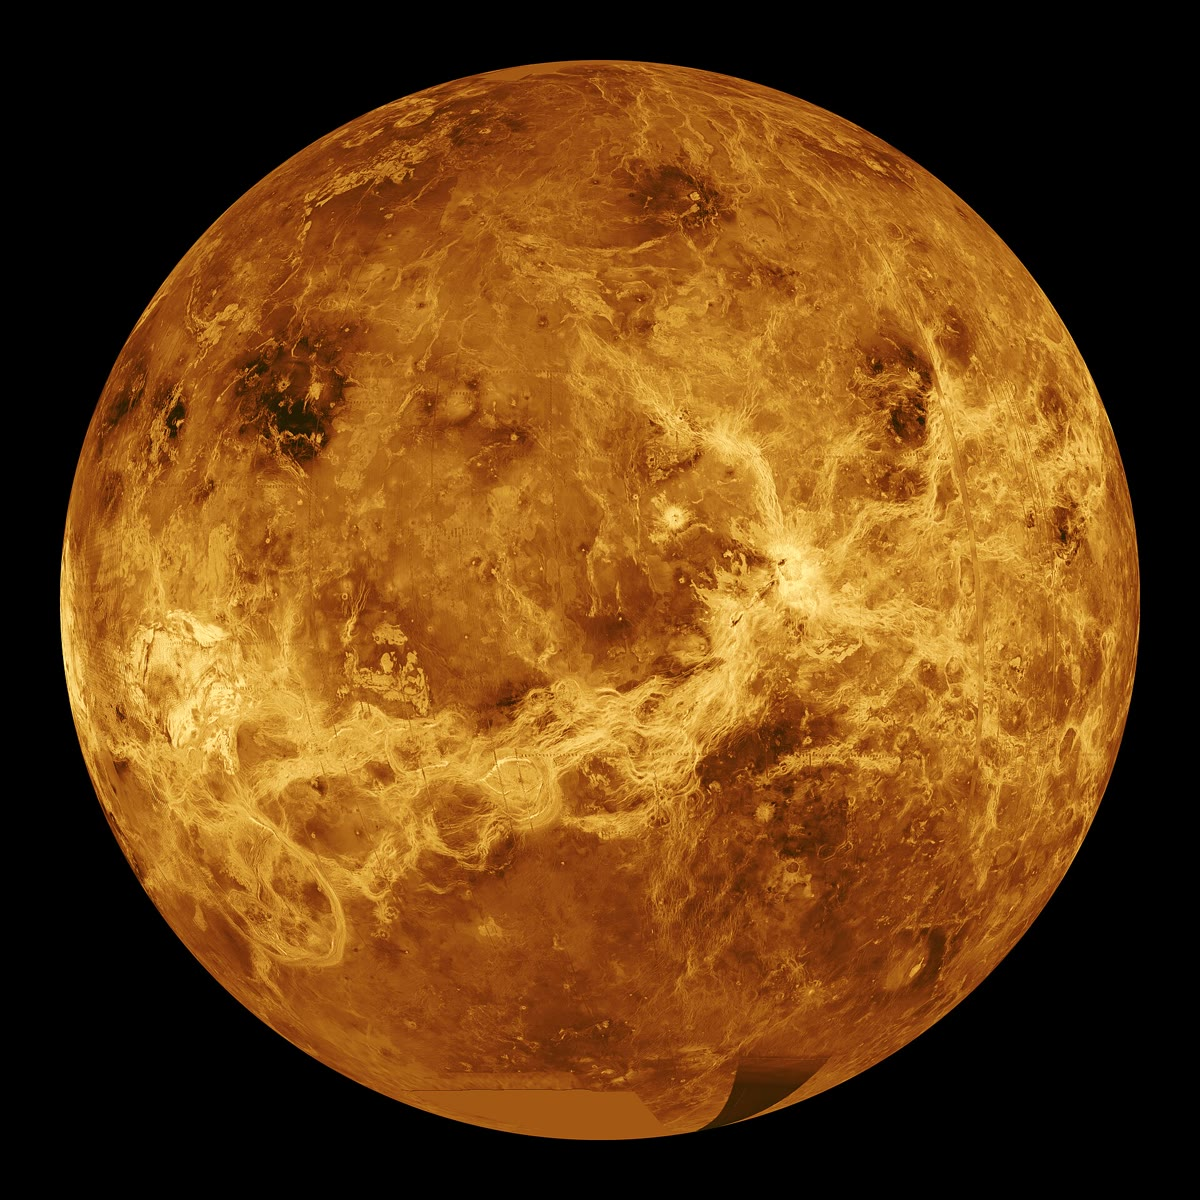
\includegraphics[width=\linewidth]{images/book3/b1-venus-radar-globe.jpg}
\end{minipage}\hspace{0.06\linewidth}
\begin{minipage}{0.4\linewidth}
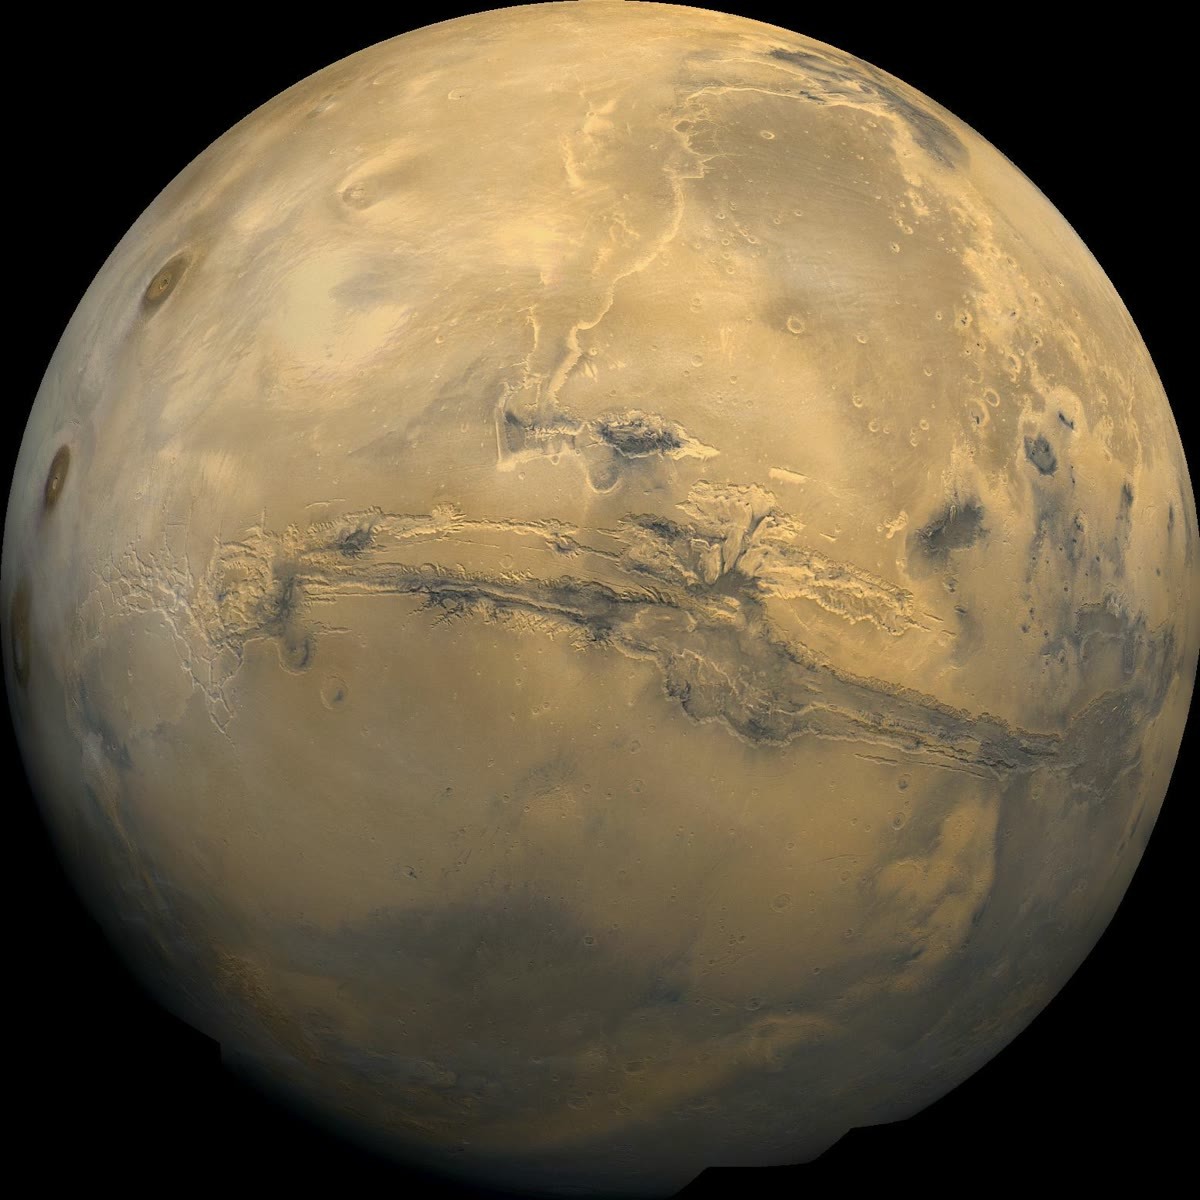
\includegraphics[width=\linewidth]{images/book3/b1-mars-valles-marineris.jpg}
\end{minipage}

{\small 左：金星表面，经麦哲伦号探测器的雷达穿透云层观测，
映射到计算机模拟的地球仪上（颜色
为模拟所得）。右：火星，由海盗 1 号轨道器拍摄，马赛克图像以
水手峡谷系统为中心。NASA/JPL 与 NASA/USGS，公有
领域。}
% ledger: commons:venus-globe, commons:mars-valles
\end{omfigure}

地表记录着塑造它们的过程。撞击坑
会在任何暴露于太空的表面上累积，因此布满撞击坑的地表，
如月球或水星的大部分表面，是古老的；而撞击坑稀少的表面
则经过了更新：或由熔岩流覆盖，或由侵蚀作用，或由把地球洋底
带回地幔的板块所更新。火山平原与
火山在所有\omterm{def:b1:comparative-planetology:planet-types}{类地行星}上都可找到。断层、裂谷
与褶皱带表明，金星与火星的岩石圈曾发生变形；
但在所有行星中，只有地球今天的岩石圈
被分割成若干以刚性块体方式运动的板块，板块生成处为洋中脊，
沉没处为海沟。地球为何独有板块构造，
至今仍有争议；水的存在会削弱岩石，是其中一种
被提出的解释。

\section{卫星与小天体}

月球直径约为地球的四分之一，作为卫星而言体积很大。其
密度 \qty{3340}{kg.m^{-3}}，接近地球地幔岩石的密度，
其\omterm{def:b1:comparative-planetology:moi}{转动惯量因子}接近 $0.4$，表明月球至多只有
一个很小的铁质地核。\omterm{def:b1:comparative-planetology:planet-types}{巨行星}拥有若干卫星系统，它们各自
本身就是一个世界（见下方照片）。木卫一是木星的四颗
大卫星中最靠内的一颗，是太阳系中火山活动最剧烈的世界，
拥有数百座火山，受木星在其上引起的潮汐加热；
火山活动更新其表面的速度快于撞击在其上留下大型撞击坑的速度。
木卫二的密度为 \qty{3010}{kg.m^{-3}}，内部为岩石，外覆冰壳，
有力证据表明冰壳之下存在一片含盐海洋。木卫三与
木卫四的密度分别为 \num{1940} 和 \qty{1830}{kg.m^{-3}}，由
数量相近的岩石与冰构成。
土卫六是土星最大的卫星，也是唯一拥有稠密大气的卫星，
大气以氮气为主，并含少量甲烷；它也是除地球外
唯一在表面拥有河流、湖泊与海洋的世界——其液体为甲烷与
乙烷；它很可能也隐藏着一片水海洋。
% ledger: planet:Moon.diameter, planet:Earth.diameter, planet:Moon.density, nasa:moon, nasa:io-facts, nasa:europa, nasa:europa-facts, nasa:ganymede, nasa:titan-facts

\begin{omfigure}
\begin{minipage}{0.4\linewidth}
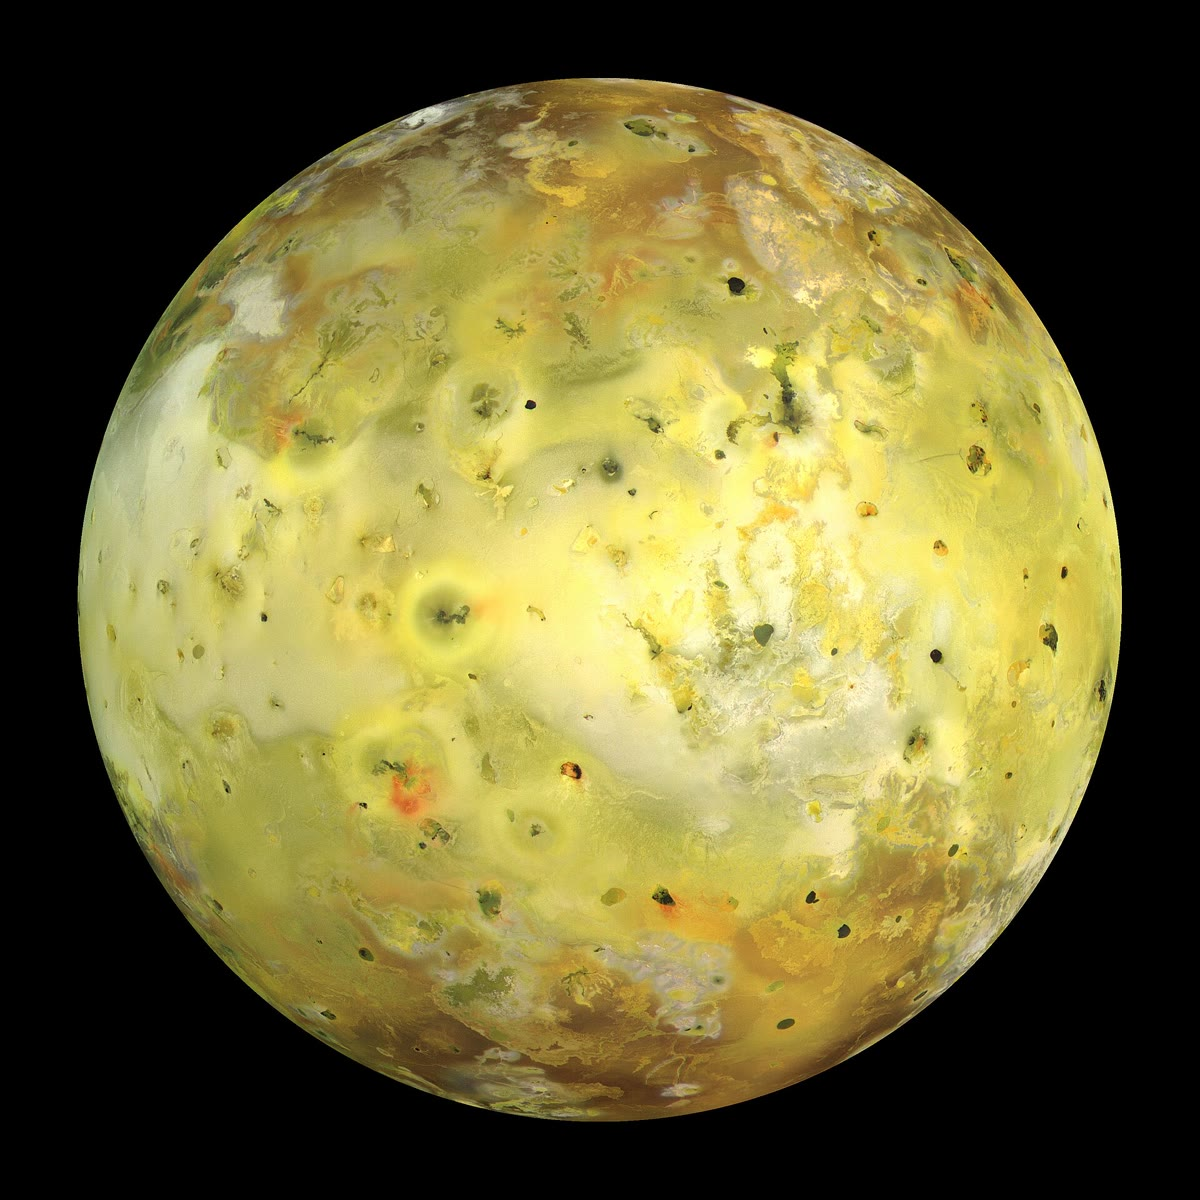
\includegraphics[width=\linewidth]{images/book3/b1-io.jpg}
\end{minipage}\hspace{0.06\linewidth}
\begin{minipage}{0.4\linewidth}
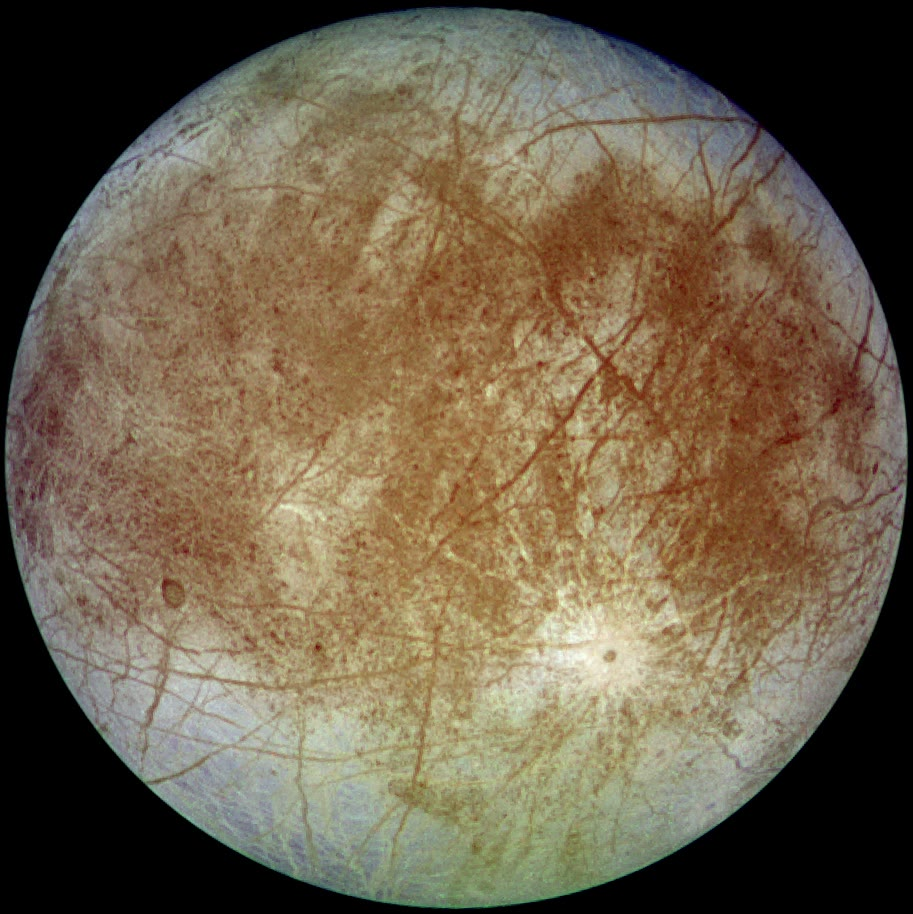
\includegraphics[width=\linewidth]{images/book3/b1-europa.jpg}
\end{minipage}

{\small 伽利略号探测器拍摄的木星两颗大卫星。左：
木卫一，表面布满火山中心，颜色由硫化合物
与熔岩所致。右：木卫二，近似自然色；长而暗的
线条是其冰壳上的裂缝。NASA/JPL/University of Arizona
与 NASA/JPL/DLR，公有领域。}
% ledger: commons:io, commons:europa, nasa:io-facts, nasa:europa
\end{omfigure}

\begin{definition}[小行星、彗星、海王星外天体]\label{def:b1:comparative-planetology:small-bodies}
\emph{小行星}\index{小行星}是绕太阳运行的小型岩质或金属质天体，
体积太小而不能称为行星，且没有彗星那样的气体与尘埃外壳；
大多数小行星位于火星与木星之间。
\emph{彗星}\index{彗星}是由冰与尘埃构成的小天体，当其
轨道使其接近太阳时，会释放出气体与尘埃，形成环绕自身的发光
外壳，并拖出背离太阳的彗尾。
\emph{海王星外天体}\index{海王星外天体}是太阳系中的一个天体，
其平均轨道位于海王星轨道之外。
\end{definition}

柯伊伯带是位于海王星之外的盘状区域，其中的\omterm{def:b1:comparative-planetology:small-bodies}{海王星外天体}
是行星形成时遗留下来的冰质与岩质天体；
冥王星自 2006 年起被划为矮行星，便是其中之一。\omterm{def:b1:comparative-planetology:small-bodies}{小行星}
则是没有形成行星的区域中的碎片。\omterm{def:b1:comparative-planetology:small-bodies}{小行星}的碎片，以及
少量来自月球与火星的物质，会以陨石的形式落到地球上。
除航天器带回的样品外，它们是我们手中仅有的其他世界样本；
其中一些自太阳系形成以来几乎未曾改变，
它们的分类，以及它们对地球成分与太阳系年龄的启示，
是本科二年级分册的内容。
% ledger: nasa:pluto-facts

\section{练习}

\begin{exercise}[$\star$]\label{exo:b1:comparative-planetology:1}
木星的质量为 \qty{1898.13e24}{kg}，平均半径为
\qty{69911}{km}。求其平均密度，并与水的密度
\qty{1000}{kg.m^{-3}} 作比较。
\end{exercise}

\begin{exercise}[$\star$]\label{exo:b1:comparative-planetology:2}
利用密度与半径图，将水星、土星、天王星和
金星分别归类为\omterm{def:b1:comparative-planetology:planet-types}{类地行星}、\omterm{def:b1:comparative-planetology:planet-types}{气态巨行星}或\omterm{def:b1:comparative-planetology:planet-types}{冰巨星}，并
依据各自的半径与密度说明理由。
\end{exercise}

\begin{exercise}[$\star$]\label{exo:b1:comparative-planetology:3}
金星接收到的辐照度为 \qty{2601.3}{W.m^{-2}}，\omterm{def:b1:comparative-planetology:albedo}{邦德反照率}为 0.77。
求其\omterm{def:b1:comparative-planetology:equilibrium-temperature}{平衡温度}。为何金星的\omterm{def:b1:comparative-planetology:equilibrium-temperature}{平衡温度}低于地球，
尽管金星比地球更靠近太阳？
\end{exercise}

\begin{exercise}[$\star$]\label{exo:b1:comparative-planetology:4}
将月球（$C = 0.394$）、火星（0.366）、地球（0.3308）、木星
（0.254）和土星（0.210）按质量分布的集中程度，由最均匀到最
集中进行排序。若一颗行星的全部质量都集中于其中心一点，
则其 $C$ 应为多少？
\end{exercise}

\begin{exercise}[$\star\star$]\label{exo:b1:comparative-planetology:5}
土卫六绕土星运行，轨道半长轴 $a = \qty{1221.87e3}{km}$，
公转周期为 \num{15.945421} 天。求土星的质量，并与表中所列的
\qty{568.32e24}{kg} 作比较。
\end{exercise}

\begin{exercise}[$\star\star$]\label{exo:b1:comparative-planetology:6}
地球在距太阳 \qty{149.6e6}{km} 处接收的辐照度为 \qty{1361}{W.m^{-2}}。
求火星（\qty{228.0e6}{km}）和木星
（\qty{778.5e6}{km}）处的辐照度，并与表中所列的
\qty{586.2}{W.m^{-2}} 与 \qty{50.26}{W.m^{-2}} 作比较。
\end{exercise}

\begin{exercise}[$\star\star$]\label{exo:b1:comparative-planetology:7}
证明：对于给定的反照率，$T_\mathrm{eq}$ 与 $d^{-1/2}$ 成正比。求
木星的 $T_\mathrm{eq}$（$S = \qty{50.26}{W.m^{-2}}$，$A = 0.343$）。
若测得木星辐射的功率大于其从太阳吸收的功率，
这对其内部意味着什么？
\end{exercise}

\begin{exercise}[$\star\star$]\label{exo:b1:comparative-planetology:8}
求金星（\qty{737}{K}）的温室增温 $T_\mathrm{surf} - T_\mathrm{eq}$，
地球（\qty{288}{K}，$A = 0.294$）与火星（\qty{214}{K}）的温室增温，
并将每一结果表示为 $T_\mathrm{eq}$ 的分数。
\end{exercise}

\begin{exercise}[$\star\star$]\label{exo:b1:comparative-planetology:9}
对于均匀球体，通过对薄球壳的转动惯量积分证明 $C = 0.4$（
薄球壳的半径为 $r$，质量为
$\mathrm dm$，其转动惯量 $\mathrm dI = \tfrac23 r^2\,\mathrm dm$）。
半径为 $R$ 的空心球壳，其值为多少？
\end{exercise}

\begin{exercise}[$\star\star\star$]\label{exo:b1:comparative-planetology:10}
水星的平均密度 $\bar\rho = \qty{5429}{kg.m^{-3}}$，$C = 0.35$，半径为
\qty{2439.7}{km}。已知地幔密度为 \qty{3300}{kg.m^{-3}}，利用
双层模型求其地核半径、地核密度以及地核质量占总质量的
比例。水星有何突出之处？
\end{exercise}

\begin{exercise}[$\star\star\star$]\label{exo:b1:comparative-planetology:11}
建立一个无大气天体的模型，其白昼半球处于均匀温度
$T_1$，夜晚半球处于 $T_2$，二者共同辐射所吸收的功率。
(a) 证明：若 $T_1^4 + T_2^4 = 2T_\mathrm{eq}^4$，则平均温度
$(T_1 + T_2)/2$ 至多为 $T_\mathrm{eq}$，且仅当
$T_1 = T_2$ 时取等号。(b) 对于月球，$T_\mathrm{eq} = \qty{270}{K}$；取
$T_2 = \qty{100}{K}$，求 $T_1$ 与平均温度。
\end{exercise}

\begin{exercise}[$\star\star\star$]\label{exo:b1:comparative-planetology:12}
金星半径为 \qty{6051.8}{km}，表面重力加速度为
\qty{8.9}{m.s^{-2}}，表面压强为 \qty{92}{bar}。求
其大气的质量，并与地球\omterm{def:b1:observing-the-sky:extinction}{大气质量} \qty{5.1e18}{kg} 作比较，
并与金星的质量 \qty{4.8673e24}{kg} 作比较。这一比较
说明地球的二氧化碳储存于何处？
% ledger: earth:Matm, planet:Venus.gravity, nasa:venus
\end{exercise}

\section{问题：称量与探测火星}

\begin{problem}[{周末问题——由火卫一求火星的质量，
以及火星的密度、温度与地核的大小}]
\label{pb:b1:comparative-planetology:1}
% ledger: nasa:phobos, nasa:mars, nasa:mars-core, const:G, const:sigma, earth:psurf, earth:gmean, planet:Mars.Prot, planet:Earth.density
% numbers computed in the scratch calculator calc/ch03.py from the rounded data
火卫一是火星较大的卫星，平均距火星中心
\qty{9378}{km}，公转周期为 \num{0.31891} 天。火星平均半径为
\qty{3389.5}{km}，自转周期为 \qty{24.6}{h}，
\omterm{def:b1:comparative-planetology:moi}{转动惯量因子} $C = 0.366$，\omterm{def:b1:comparative-planetology:albedo}{邦德反照率}为 0.250，表面平均压强为 \qty{6.36}{mbar}；
它从太阳接收 \qty{586.2}{W.m^{-2}}，
表面平均温度约为 \qty{214}{K}。火卫一的质量为
\qty{1.06e16}{kg}。取 $G = \qty{6.6743e-11}{m^3.kg^{-1}.s^{-2}}$
和 $\sigma = \qty{5.6704e-8}{W.m^{-2}.K^{-4}}$。

\medskip
\noindent\textbf{第一部分——称量火星。}
\begin{enumerate}
  \item 将火卫一的周期换算为秒。
  \item 求火星的 $GM$。
  \item 由此求火星的质量。
  \item 忽略火卫一的质量是否合理？
  \item 求火卫一的轨道速度。
  \item 比较火卫一的周期与火星的自转周期。火卫一
        在火星天空中沿哪个方向穿过？
\end{enumerate}

\medskip
\noindent\textbf{第二部分——密度与重力。}
\begin{enumerate}[resume]
  \item 求火星的体积。
  \item 求火星的平均密度，精确到 \qty{10}{kg.m^{-3}}。
  \item 与地球的平均密度 \qty{5514}{kg.m^{-3}} 作比较，给出地球密度更大的
        两个原因。
  \item 求火星表面的重力加速度。
  \item 求火星表面的逃逸速度。
\end{enumerate}

\medskip
\noindent\textbf{第三部分——温度与大气。}
\begin{enumerate}[resume]
  \item 求火星的\omterm{def:b1:comparative-planetology:equilibrium-temperature}{平衡温度}。
  \item 将其与火星表面的平均温度作比较，温室增温
        有多大？
  \item 求火星每平方米表面之上大气的质量，
        并与地球的相应值作比较（$p = \qty{1014}{hPa}$，
        $g = \qty{9.82}{m.s^{-2}}$）。
  \item 求火星大气的总质量。
  \item 火星大气的 \qty{95}{\percent} 为二氧化碳，
        但其温室增温很小。试说明原因。
\end{enumerate}

\medskip
\noindent\textbf{第四部分——火星的地核。}
\begin{enumerate}[resume]
  \item 若火星为均匀天体，$C$ 应为多少？所测得的
        数值说明了什么？
  \item 用相对地核半径 $x$、地幔密度 $\rho_m$
        和地核密度 $\rho_c$，
        写出双层火星模型的平均密度。
  \item 用同样的量写出其\omterm{def:b1:comparative-planetology:moi}{转动惯量因子}。
  \item 证明 $x^2 = (\tfrac52C\bar\rho - \rho_m)/(\bar\rho - \rho_m)$。
  \item 利用第 8 题中的平均密度，并取 $\rho_m =
        \qty{3500}{kg.m^{-3}}$，求 $x$ 与地核密度。
  \item 火星质量中有多大比例位于地核之中？
  \item 对 $\rho_m = 3450$ 与
        \qty{3550}{kg.m^{-3}}，重做第 21 题。由此
        可对模型的精度得出什么结论？
  \item 由 $\rho_m = \qty{3500}{kg.m^{-3}}$ 的模型，求火星地核的半径，
        并与行星数据表中的值 \qty{1830}{km} 作比较，
        再与近期地震学结果 \qty{1650}{km} 至
        \qty{1675}{km} 作比较。
\end{enumerate}
\end{problem}
